\chapter{Grundlagen der Signalverarbeitung}

Ein \emph{Signal} ist eine Funktion eines Parameters mit numerischen Wertebereich. Die Abbildung zwischen Defintions- und Wertebereich kann, aber muss nicht durch eine Formel definiert sein. So fällt $f(x) = \sin( x )$ genauso unter die Definition eines Signals wie eine Folge numerischer Werte, die durch die Aufnahme eines Messgerätes enstanden sind. Weiterhin kommt dem Wertebereich eine gewissen Bedeutung zu, wie \emph{Zeit} oder \emph{Ort}. Ein typisches Beispiel für ein Signal ist die Spannung, die abhängig von der Zeit von einem Mikrofon erzeugt wird.  Da in dieser Arbeit nur Signale von Bedeutung sind, deren Wertebereich sich auf die Zeit bezieht, konzetrieren sich alle folgenden Bereich auf diesen Bereich- Im Zusammenhang mit Signalen wird der Definitionsbereich auch als \emph{unabhängiger Parameter} und der Wertebereich auch als \emph{abhängiger Parameter} bezeichnet. \cite[S. 11-12]{dspGuide} \cite[S. 22-23]{dspMichigan}

 Bei einem zeit-kontinuierlichen Signal $x( t )$ ist der Wertebereich kontinuierlich, wie in Formel  \ref{eq:time-cont-signal} definiert. Bei einem zeit-diskreten Signal $x[n]$ ist der Wertebreich diskret, wie in Formel \ref{eq:time-disc-signal} definiert. So beschreibt beispielsweise $x[17] = s$ den Wert zur Zeit $n = 17$. \glqq Zeit\grqq{} hat in diesem Kontext keine Einheit. Ein Wert wird auch als \emph{Sample} oder \emph{Amplitude} bezeichnet. $x[17] $ meint somit das 17. Sample des Signals. Abbildung \ref{img:aSignal} zeigt Beispiele für ein zeit-kontinuierliches und ein zeit-diskretes Signal. \cite[S. 22 - 23]{dspMichigan}

 \begin{equation}
x(t) = s \; , t \in \mathbb{R}
\label{eq:time-cont-signal}
\end{equation}


\begin{equation}
x[n] = s \; , n \in \mathbb{Z} 
\label{eq:time-disc-signal}
\end{equation}

\begin{figure}
	\centering
	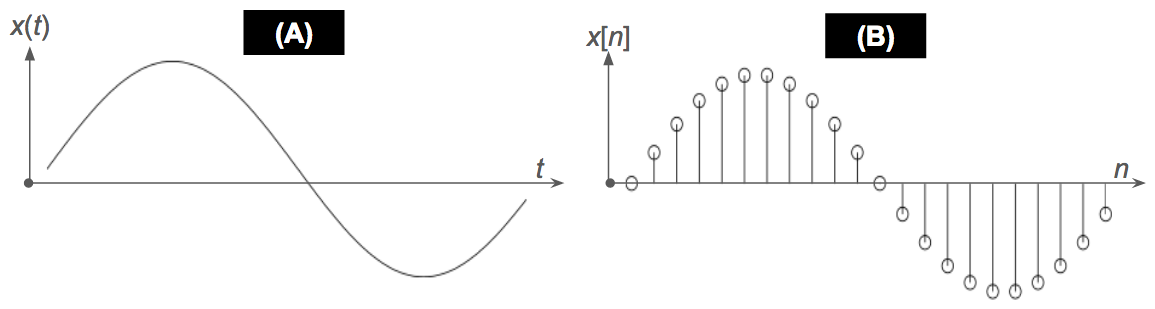
\includegraphics[width=0.7\textwidth]{bilder/aSignal02.png}
	\caption{Ein zeit-kontinuierliches Signal (A) und ein zeit-diskretes Signal (B)}
	\label{img:aSignal}
\end{figure}

Zeit-diskrete Signale werden häufig dadurch gewonnen, dass ein zeit-kontinuierliches Signal in regelmäßigen Intervallen abgetastet wird. Dieser Prozess wird als \emph{Sampling} bezeichnet und durch Formel \ref{eq:sampling} definiert. Der Parameter $T_s$ wird als \emph{Sampling-Interval} bezeichnet. Das Reziproke $\frac{1}{T_s} = f_s$ heißt \emph{Sampling-Rate} und wird in der Einheit $\frac{1}{\text{s}} = \text{Hz}$. Eine Sampling-Rate von $f_s = \SI{44100}{\hertz}$ bedeutete beispielsweise, dass ein Signal 44100 mal pro Sekunde abgetastet wurde.\cite[S. 24]{dspMichigan}

\begin{equation}
x[n] = s(n \cdot T_s) \; , -\infty < n < \infty
\label{eq:sampling}
\end{equation}
	
Da in dieser Arbeit nur zeit-diskrete Signale von Interesse sind, werden ab diesem Punkt die Definitonen für zeit-kontinuierliche Signale ausgelassen. Der \emph{Support} ist das kleinst mögliche Zeitintervall, der alle Samples enthält, die nicht den Wert 0 haben, wie Formel \ref{eq:support} definiert. Die \emph{Dauer} eines Signales ist die Länge des Supportes nach Formel . Das Signal $x[n] = \cos(n) \: ,0\leq n \leq 3$ hat beispielsweise den Support $[0,3] = \{0,1,2,3\} $ und die Dauer $4$. Ein \emph{unendliches Signal} hat einen unendlichen langen Support, das heißt es gilt Duration$(x) = \infty$. Ein \emph{endliches Signal} hat einen endlichen Support, das heißt Duration$(x) \neq\infty$. \cite[S. 24]{dspMichigan}

\begin{equation}
\label{eq:support}
\begin{split}
\text{Sup}(x) = [sup_s, sup_e] \quad , sup_s, sup_e \in \mathbb{Z} \\,  x[sup_s] \neq 0 \:  \wedge \:  x[sup_e] \neq 0 \: \wedge \: \forall n \
\not\in [sup_s, sup_e] : x[n] = 0
\end{split}
\end{equation}

\begin{equation}
\text{Duration}(x) = sup_e - sup_s + 1
\label{eq:duration}
\end{equation}

Ein Signal gilt als \emph{periodisch}, wenn Formel \ref{eq:periodicity} erfüllt ist. Der Parameter $N$ wird als \text{Periode} von $x$ bezeichnet. Wenn ein Signal mit $N$ periodisch ist, dann ist es auch mit $2N, 3N, \ldots $ periodisch. Die Grundfrequenz $N_0$ ist das kleinste N, für das Formel \ref{eq:periodicity} erfüllt ist. Abbildung \ref{img:periodicSic} zeigt ein Beispiel für ein nicht-periodisches und ein periodisches Signal. \cite[S. 24]{dspMichigan}

\begin{equation}
\exists N : \forall n \in Sup : x[n+N] = x[n] \rightarrow \text{Periodisch}(x,N) = true
\label{eq:periodicity}
\end{equation}

\begin{figure}[h]
	\centering
	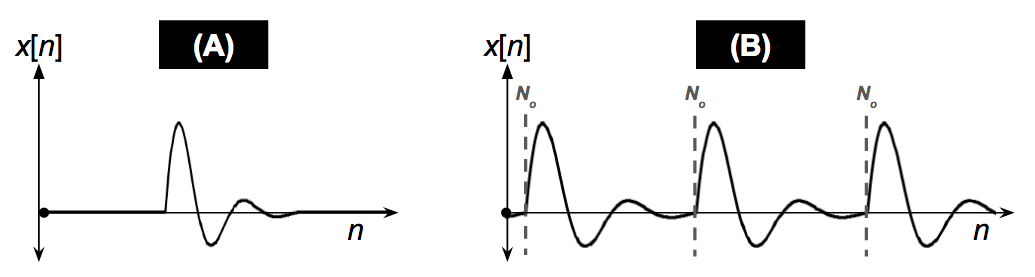
\includegraphics[width=0.7\textwidth]{bilder/periodicSig.png}
	\caption{Ein nicht-periodisches Signal (A) und ein periodisches Signal (B)}
	\label{img:periodicSic}
\end{figure}

\section{Statistische Merkmale}

Im folgenden wird ein überblick über die häufig verwendete Signaleigenschaften gegeben. Abbildung \ref{img:sigStats} visualisiert die Erläuterungen.

\begin{enumerate}[leftmargin=*]
	
\item Der \textbf{Maximalwert / Minimalwert} beschreibt den höchsten / niedrigsten in  $x$ enthaltenen Wert nach den Formel $\max(x)$ und $\min(x)$.
	
\item Der \textbf{Durchschnittswert / Average Value} beschreibt den durchschnittlichen Wert aller Samples von $x$ nach Formel \ref{eq:avg}. Dieser Durchschnittswert wird über dem Intervall $[n_1, n_2]$  berechnet.

\begin{equation}
\text{AVG}(x) = \frac{1}{n_2 - n_1 + 1} \sum_{n = n_1}^{n_2} x[n]
\label{eq:avg}
\end{equation}

\item Der \textbf{Mean Squared Value} (\emph{MSV}) beschreibt den quadrierten Durchschnittswert über eine bestimmtes Interval nach Formel \ref{eq:msv}. Er wird auch als \emph{durchschnittliche Energie} oder \emph{average Power} bezeichnet.

\begin{equation}
\text{MSV}(x) = \frac{1}{n_2 - n_1 + 1} \sum_{n = n_1}^{n_2} x[n]^2
\label{eq:msv}
\end{equation}

\item Das \textbf{Root Mean Square} (\emph{RMS}) ist die Wurzel des Mean Squared Value nach Formel\ref{eq:rms}. Der RMS findet häufiger Anwendung als der MSV, da er besser ins Verhältnis zu den Werten des Signals gesetzt werden kann. Er wird im Deutschen auch als \textbf{Effektivwert} oder \textbf{Durchschnittsleistung} bezeichnet. Da die deutschen Begriffe in einigen Quellen jedoch auch für den MSV verwendet werden, wird an dieser Stelle nur mit den englischen Begriffen gearbeitet.

\begin{equation}
\text{RMS}(x) = \sqrt{\frac{1}{n_2 - n_1 + 1} \sum_{n = n_1}^{n_2} x[n]^2}
\label{eq:rms}
\end{equation}

\item Die \textbf{Energie / Energy} bezeichnet die \glqq Stärke \grqq{} eines Signals über einen bestimmten Intervall nach Formel \ref{eq:energy}. Sie entspricht dem MSV-Wert multipliziert der Länge des Intervalls. \cite[S. 27-28]{dspMichigan}

\begin{equation}
\text{E}(x) = \sum_{n = n_1}^{n_2} x[n]^2
\label{eq:energy}
\end{equation}
	
\end{enumerate}	

\begin{figure}[h]
	\centering
	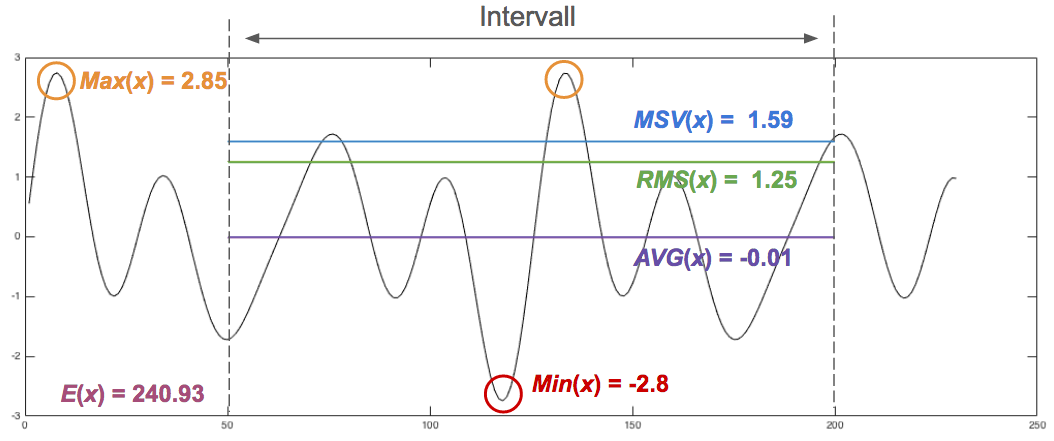
\includegraphics[width=0.7\textwidth]{bilder/sigStats.png}
	\caption{Statistische Werte eines Signals über das Intervall [50,200]}
	\label{img:sigStats}
\end{figure}

Die Addition und Multiplikation wird bei Signalen komponentenweise durchgeführt, das heißt $x_1[n] + x_2[n] = y[n] $ und $x_1[n] \cdot x_2[n] = y[n] $. Abbildung \ref{img:addAndMultSig} visualisiert diese Operationen. 

\begin{figure}[h]
	\centering
	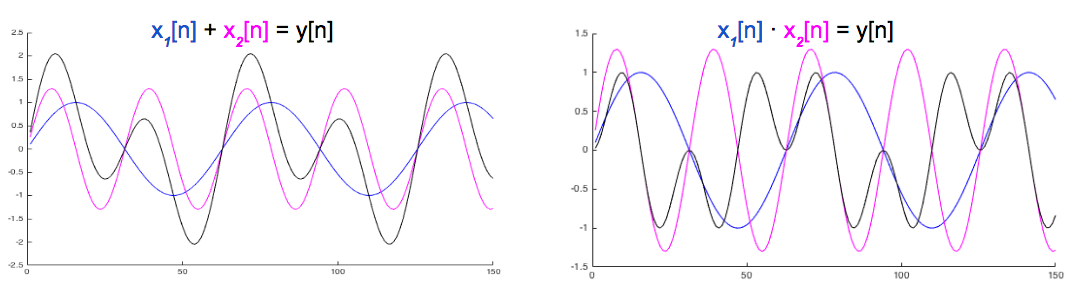
\includegraphics[width=0.8\textwidth]{bilder/addAndMultSig.png}
	\caption{Komponentenweise Addition und Mulitplikation zweier Signale}
	\label{img:addAndMultSig}
\end{figure}

\section{Fehlersignale}

Die Addition wird unter anderem für die Modellierung des Einflusses von Störungen benötigt. Angenommen, ein Signal $x$ wird übertragen, auf dem Übertragungsweg jedoch durch ein anderes Störsignal wie z.B. Rauschen $e$ überlagert. Dieses Störsignal wird in diesem Zusammenhang auch als \glqq{Fehler-Signal} bezeichnet. Das resultierende Signal $x'$ wird nach Formel \ref{eq:sigErrorAddition} berechnet. Kennt man sowohl das Eingangssignal $x$ als auch das Ausgangssignal $x'$, kann das Störsignal $e$ nach Formel \ref{eq:calErrorSig} berechnet werden.

\begin{equation}
x'[n] = x[n] + e[n]
\label{eq:sigErrorAddition}
\end{equation}

\begin{equation}
e[n] = x'[n] -x[n]
\label{eq:calErrorSig}
\end{equation}

 Errechnet man nun den den MSV- oder RMS-Wert des Störsignales $e$, gibt das Ergebnis einen Eindrück über die \glqq Stärke \grqq{} des Fehler-Signals. Der MSE-Wert des Fehlers wird in diesem Zusammenhang auch als \emph{Mean Squared Error} (\emph{MSE}) und der RMS-Wert als \emph{Root Mean Squared Error} (\emph{RMSE}) oder einfach als \emph{Fehler} oder \emph{Error} bezeichnet. Formel\ref{eq:mse} und \ref{eq:error} definierten die Berechnungen des MSE und RMSE. Der RMSE hat im Gegensatz zum MSE den Vorteil, dass er besser ins Verhältnis zu den Werten des Fehlersignals gestetzt werden kann. Ein RMSE $= 0$ heisst, dass $x = x'$ und somit kein Störsignal vorliegt. Ein RMSE = RMS$(x)$ heisst, dass Eingangs- und Störsignal den selben Effektivwert und somit die selbe \glqq stärke\grqq{} besitzen. Abbildung \ref{img:snrStuff} visualisiert die Berechnung des MSE und RMSE. \cite[S: 28 - 29]{dspMichigan}

\begin{equation}
\text{MSE}(x,x') = \frac{1}{n_2 - n_1 + 1} \sum_{n = n_1}^{n_2} (x[n]-x'[n])^2
\label{eq:mse}
\end{equation}

\begin{equation}
\text{RMSE}(x,x') = \sqrt{\frac{1}{n_2 - n_1 + 1} \sum_{n = n_1}^{n_2} (x[n]-x'[n])^2}
\label{eq:error}
\end{equation}

Eine weitere Betrachtungsweise bezüglich der Stärke des Rauschens auf das Signal ist, das Eingangssignal ins Verhältnis zum Rauschsignal zu setzen. Formel \ref{eq:snrPre} gibt die Definition. Ein SNR\textsubscript{rel}$(x,e) = 1$ heißt, dass das Eingangssignal den selben MSV wie das Fehlersignal hat. Meistens ist der MSV des Eingangssignals in der Praxis sehr viel höher als der des Fehler-Signals. Um den Zahlenraum zu begrenzen, wird die Pseudo-Einheit dB verwendet. Formel \ref{eq:snrDb} den so berechneten \emph{Signal-Rausch-Abstand} (\emph{SNR}, englisch Signal-to-Noise-Ratio). Entgegen des MSE weisst ein \emph{niedriger} SNR-Wert auf ein \emph{starkes} Rauschen hin, und ein \emph{hoher} SNR auf ein \emph{schwaches} Rauschen! Abbildung \ref{img:snrStuff} visualisiert die Berechnung des SNR.

%% To do: Gute Quelle suchen!!

\begin{equation}
\text{SNR}_{rel}(x,e) = \frac{MSV(x)}{MSV(e)}
\label{eq:snrPre}
\end{equation}

\begin{equation}
\text{SNR}(x,e) = 10 \cdot  \lg \Big(\frac{MSV(x)}{MSV(e)} \Big) \text{ dB}
\label{eq:snrDb}
\end{equation}

\begin{figure}[h]
	\centering
	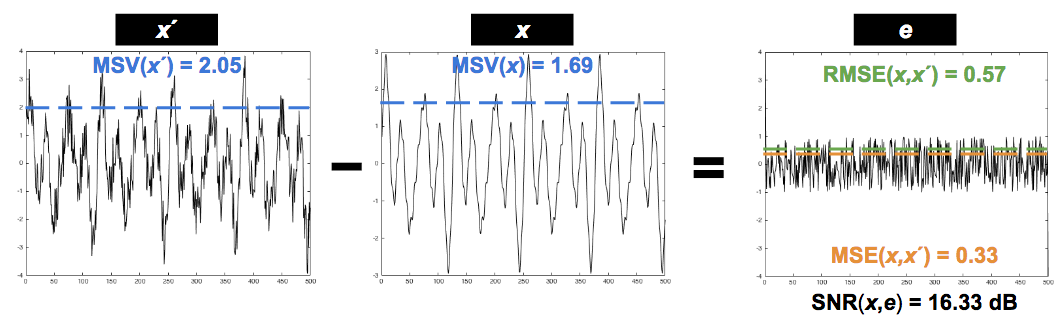
\includegraphics[width=1\textwidth]{bilder/snrStuff02.png}
	\caption{Berechnung des MSE, RMSE und SNR eines von Rauschen gestörten Signals}
	\label{img:snrStuff}
\end{figure}

\section{Korrelation}

Die \emph{Korrelation} (engl \emph{Correlation}) zweier Signale $x_1$ und $x_2$ wird nach Formel \ref{eq:correlation} als die Summe aller Samples des Produktes der beiden Signale über einen bestimmtes Intervall $[n_1, n_2]$ definiert. Das Ergebnis ist eine Wert $\in \mathbb{R}$ welches die \glqq Ähnlichkeit der beiden Signale\grqq{} kennzeichnet. Ein Positiver Wert weisst auf eine \emph{positive Korrelation} hin, ein negativer Wert auf eine \emph{negative Korrelation}, und ein Wert von $\text{Corr}(x_1,x_2) = 0$ auf \emph{keine Korrelatoin}. Aus der größe des Wertes kann die Stärke der Korrelation jedoch nicht direkt interpretiert werden. Bei der \emph{normalisierten Korrelation} Corr$_N(x,y)$ wird daher die Korrelationswert ins Verhältnis zu den Energien der beiden Signale gesetzt, wie in Formel \ref{eq:normCorrelation} definiert. Der Wertebereich der normalisierten Autokorrelation  ist $-1 \leq \text{Corr}_N(x,y) \leq +1$. Daraus ergeben sich die in Formel \ref{eq:correlationProps} definierten Zusammenhänge. Ein Wert von $ \text{Corr}_N(x,y) = 1$ wird auch als \emph{perfekte Korrelation} bezeichnet, ein Wert von  $ \text{Corr}_N(x,y) = -1$ als \emph{anti-perfekte Korrelation} \cite[S. 46 - 47]{dspMichigan} Abbildung \ref{img:corrSigsComp} visualisiert die normalisierte Korrelation eines Signales $x$ mit den Signalen $y_n$.

\begin{equation}
\text{Corr}(x,y) = \sum_{n=n_1}^{n_2} x[n] \cdot y[n]
\label{eq:correlation}
\end{equation}

\begin{equation}
\text{Corr}_N(x,y) = \frac{\text{Corr}(x,y)}{\sqrt{\text{E}(x) \cdot \text{E}(y)}}
\label{eq:normCorrelation}
\end{equation}

\begin{equation}
\text{Corr}_N(x,y) = 
\begin{cases}
1  \quad \rightarrow  x = y \\
-1 \; \rightarrow x = -y
\end{cases}
\label{eq:correlationProps}
\end{equation}

\begin{figure}[h]
	\centering
	\includegraphics[width=1\textwidth]{bilder/corrSigsComp.png}
	\caption{Correlation der Signale $x$ und $y$}
	\label{img:corrSigsComp}
\end{figure}

Die Korrelation und die normalisierte Korrelation werden aufgrund ihrer Eigenschaften verwendet, um ein Signal $x$ in einem Signal $y$ zu detektieren. Häufig ist das Ziel, ein von einem Rauschen $e$ überlagerten Signal $x+e = y$ auf das Vorhandensein des erwarteten Signales $x$ hin zu überprüfen. Wie in Abbildung \ref{img:corrSigsComp} zu sehen ist, ist der Korrelationswert jedoch von der Verzögerung des Signals abhängig. Daher wird in der $Cross-Correlation$ das Signal $y$ mit einer verzögerten Varianten des Signals $x$ korreliert, wie in Formel \ref{eq:XCorr} definiert. Der parameter $k$ wird als \emph{Lag} bezeichnet und gibt die Verzögerung an. 

\begin{equation}
\text{X-Corr}(x,y,k) = \sum_{n=-\infty}^{\infty} x[n-k] \cdot y[n]
\label{eq:XCorr}
\end{equation}

Im Prozess der so genannten \emph{Running Correlation} nutzt man die Cross-Correlation mit den Lags $k = 0 \cdots k_{max}$ zur Erstellung des \emph{Korrelationssignals} $r$, wie in Gleichung \ref{eq:runningCorrelation} definiert. Das Signal $r$ gibt Auskunft, zu welchen Verzögerungswerten $k$ die größten Ähnlichkeiten zwischen $x$ und $y$ gefunden wurden. 

\begin{equation}
r[k] = \text{X-Corr}(x,y,k) \quad, k = 0 , \ldots , k_{max} 
\label{eq:runningCorrelation}
\end{equation}

Abbildung \ref{img:slidingCorrelation} zeigt ein Beispiel für die Erzeugung von $r$ mit der Sliding Correlation. (A) zeigt das zu detektierende Signal $x$ und (B) das Signal $y$. (C) zeigt das Korrelationssignal $r$ mit den Lags $k = 1, \ldots ,1150$ \cite[S. 47 - 48]{dspMichigan}

\begin{figure}[h]
	\centering
	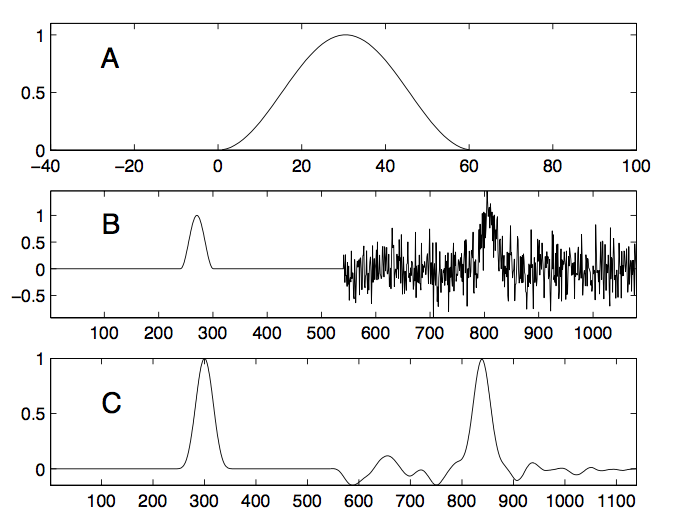
\includegraphics[width=0.5\textwidth]{bilder/slidingCorrelation.png}
	\caption{Beispiel einer Running Correlation}
	\label{img:slidingCorrelation}
\end{figure}

\section{Faltung}

Die \emph{Faltung} (engl. \emph{Convolution}) ist eine der Zentralen Operationen zwischen zwei Signalen, so wie die Addition oder die Mulitplikation. Sie wird mit dem Symbol $*$ notiert. Sie wird notiert mit $x* h = y$. 

Die Faltung basiert auf der \emph{Faltungs-Summe}, welche die Faltung zunächst Punktweise definiert. Die Gleichung wird in Formel \ref{eq:convolutionSum} abgebildet. In diesem Zusammenhang wird $x$ Eingangs- und $y$ als Ausgangs-Signal bezeichnet. Je nach Anwendungsfall bekommt $h$ den Namen \emph{Faltungs-Kernel}, \emph{Filter-Kernel} oder einfach \emph{Kernel}. \cite[S. 107-108]{dspGuide}

\begin{equation}
y[n] = x[n] * h[n] = \sum_{i=1}^{M} h[n] * x[i-n]
\label{eq:convolutionSum}
\end{equation}

Das Ergebnis einer Berechneten Faltungssumme nach \ref{eq:convolutionSum} ist ein einzelner Wert. Wird die Faltungs-Summe ähnlich der Cross-Correlation für $n = 1...N+M-1$ durchgeführt, ist das Ergebnis ein Signal. Die tatsächliche Faltung wird in Gleichung \ref{eq:convolution} definiert. $x$ ist ein Signal mit Support$(x) = [1,N]$ und Duration$(x) = N$, $h$ ist ein Signal mit Support$(x) = [1,M]$ und Duration$(h) = M$ und $y$ ist ein Signal mit Support$(y) = [1,N+M-1]$ und Duration$(y) = N+M-1$. Das heißt, dass das Eingangssignal um die Länge des Faltungskerns verlängert wird. Abbildung 	\ref{img:convolutionExample} zeigt ein Beispiel für die Faltung.\cite[S. 115-120]{dspGuide}

\begin{equation}
y = x * h = \big[ \: x[1] * h[1] , \ldots , x[N+M-1] * h[N+M-1] \: \big]
\label{eq:convolution}
\end{equation}

\begin{figure}[h]
	\centering
	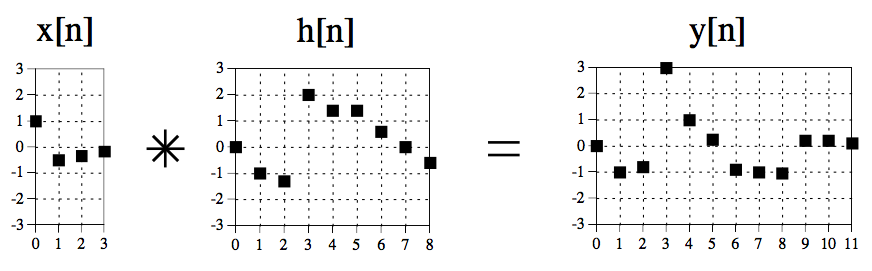
\includegraphics[width=0.8\textwidth]{bilder/convolutionExample.png}
	\caption{Beispiel für die Faltung}
	\label{img:convolutionExample}
\end{figure}

Das neutrale Element der Faltung ist der \emph{Delta-Funktion}, definiert in Gleichung \ref{eq:delta} . Das heißt, dass $x * \delta = x$ . Die Faltung ist kommutativ, das heißt $ x * h = h * x = y$ . \cite[S. 107, 113 ]{dspGuide}

\begin{equation}
\delta[n] = 
\begin{cases}
1 \quad , n = 0\\
0 \quad ,  n \neq 0
\label{eq:delta}
\end{cases}
\end{equation}


\section{Diskrete Fourier-Transformation}

\section{Filter}
\section{akustische Modellierung der menschlichen Stimme}
\section{Feststellung von Periodizität in Signalen}
\subsection{Zero-Crossing-Rate}
\subsection{Methoden des Frequenzbereiches}
\subsection{Autokorrelation}
\subsection{Cepstrum}